%%%%%%%%%%%%%%%%%%%%%%%%%%%%%%%%%%%%%%%%%%%%%%%%%%%
%% P3: Phenomenology of Particle Physics                         
%%
%% Author:  André Rubbia                   		 
%%
%% Figure 11.16 Differential cross-section for $e^+e^- \rightarrow\gamma\gamma$ at high energies.
%%
%% This work is licensed under the Creative Commons Attribution 4.0 International License. 
%% To view a copy of this license, visit http://creativecommons.org/licenses/by/4.0/ or 
%% send a letter to Creative Commons, PO Box 1866, Mountain View, CA 94042, USA.
%%
%%%%%%%%%%%%%%%%%%%%%%%%%%%%%%%%%%%%%%%%%%%%%%%%%%%

\documentclass[a4paper,10pt]{article}

\usepackage[T1]{fontenc}
\usepackage[utf8]{inputenc}
\usepackage{lmodern}
\usepackage[labelfont=bf]{caption}
\usepackage{upgreek}

\usepackage{tikz}
\usepackage{pgfplots}
\pgfplotsset{compat=1.17}
\usepgfplotslibrary{ternary}
\usepgfplotslibrary{fillbetween}
\usepgfplotslibrary{external}

\usepackage{braket}

\def\d{\mathrm{d}}

\begin{document}

%%%%%%%%%%%%%%%%% FIGURE %%%%%%%%%%%%%%%%%%%%%%%%%%%%%%%%%%
\begin{figure}[htb]
\begin{center}
\pgfplotsset{every axis/.append style={
    font=\large,
    line width=1pt,
    tick style={line width=0.8pt}}}
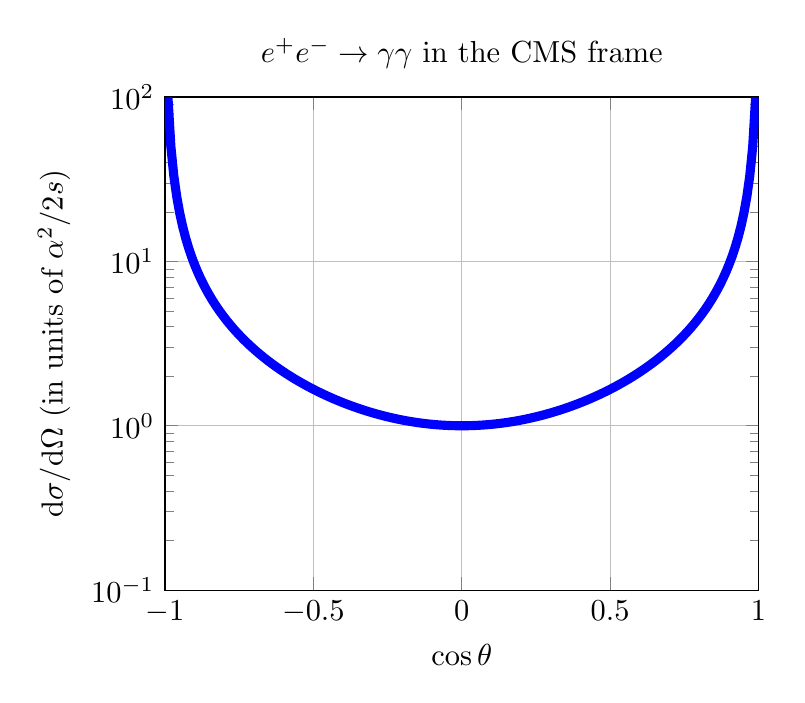
\begin{tikzpicture}[scale=1.1]
    \begin{semilogyaxis}[
        title=$e^+e^- \rightarrow\gamma\gamma$ in the CMS frame,
        xlabel={$\cos\theta$},
        ylabel={$\d\sigma/\d\Omega$ (in units of $\alpha^2/2s$)},
        xmin=-1, xmax=1,
        ymin = 1e-1,
        ymax=100,
        minor y tick num=1,
                        grid = major
    ]
        \addplot [blue,samples=201,  line width=3pt, domain=-0.99:0.99] {(1+x^2)/(1-x^2)};
   \end{semilogyaxis}
\end{tikzpicture}%
\caption{Differential cross-section
for $e^+e^- \rightarrow\gamma\gamma$ at high energies.}
\end{center}
\end{figure}
%%%%%%%%%%%%%%%%% END FIGURE %%%%%%%%%%%%%%%%%%%%%%%%%%%%%%
%

\end{document}
